% Based on the supplied JAIST thesis_J.tex (2022-02 revised).
% Requires pLaTeX + pBibTeX + dvipdfmx. Do not use XeLaTeX/Tectonic.
% v7: IPAex TrueType fonts (Docker map), explicit Adobe-Japan1 ToUnicode in build.py.
\documentclass[dvipdfmx,12pt,a4j]{jreport}
\usepackage[T1]{fontenc}
\usepackage{lmodern}
\usepackage[dvipdfmx]{graphicx}
\usepackage[margin=23mm,top=25mm,bottom=25mm]{geometry}
\usepackage{array,booktabs,float,listings,textcomp,url}
\usepackage{xcolor,tikz}
\usepackage[dvipdfmx,hidelinks]{hyperref}
\usepackage{pxjahyper}
\usetikzlibrary{arrows}
\AtBeginDvi{\special{pdf:tounicode EUC-UCS2}}
\counterwithout{figure}{chapter}
\counterwithout{table}{chapter}
\renewcommand{\thefigure}{\arabic{figure}}
\renewcommand{\thetable}{\arabic{table}}
\lstset{basicstyle=\ttfamily\fontsize{9}{11}\selectfont,
  columns=fullflexible,keepspaces=true,showstringspaces=false,
  breaklines=true,breakatwhitespace=false,breakindent=4em,
  frame=tb,framerule=.3pt,upquote=true,aboveskip=.7em,belowskip=.7em}
\hypersetup{pdftitle={2コアCPUにおける分割ソートの設計と検証},pdfauthor={早坂（正式氏名未確定）}}
\hypersetup{pageanchor=false}
\begin{document}
\thispagestyle{empty}
\begin{center}
副テーマ実施報告\\
\vfill
{\LARGE 2コアCPUにおける\\分割ソートの設計と検証}\\
\bigskip
共有メモリの調停と完了同期を実コードと波形で確認する\\
\vfill
早坂（正式な氏名表記は未確定）\\
学籍番号：未確定\\
\vfill
主指導教員：未確定\\
\vfill
北陸先端科学技術大学院大学\\
所属の正式表記：未確定\\
\vfill
\number\year 年\number\month 月\\
改訂日：2026年11月22日\\
\vfill
\end{center}
\clearpage\pagestyle{empty}
\centerline{Abstract}\bigskip
This report integrates an existing two-core CPU, sorting programs, and test
code, and verifies their behavior and cycle counts using XSim 2023.1.
The cores sort separate halves of an array; Core0 merges the results after
both cores publish completion. A ten-element execution is traced using
source-code excerpts and recorded waveforms, connecting synchronization,
shared-port contention, and the final array. All 54 conditions, comprising
18 input groups and three execution modes, passed the output and intermediate
state checks. Compared with executing the same split-and-merge work on one
core, the cycle count decreased from 442 to 366 for the specified ten-element
input, and from 8,614 to 5,527 for a fixed random 64-element input.
Initial copying and merging remain on Core0, and shared-port stalls also
remain, so the total cycle count was not halved. The results concern RTL
simulation; synthesis and physical FPGA performance were not evaluated.
\clearpage
\centerline{概要}\bigskip
共有メモリを使う2コアCPUで分割ソートの動作を検証した。各コアが配列の半分をバブルソートし、両コアのソートが終わるとCore0が結果をマージする。
既存のCPU、ソート生成器、テストベンチを組み合わせ、入力ROMの読出し経路とコアIDの互換アドレスを加えた。
XSim 2023.1で18の入力群をそれぞれ3方式で実行した。全54条件で、出力と実行途中の状態が検査に合格した。
10要素の波形では、共有ポートの競合でCore1が停止する区間と、両側のソート完了からマージを経て最終配列が得られるまでを追った。

同じ分割ソートとマージを1コアで順に行う場合に比べ、指定の10要素では442から366サイクル、固定乱数64要素では8,614から5,527サイクルに減った。
初期コピーとマージはCore0が担当し、並行ソート中にも共有ポートの待ち時間がある。
評価はRTLシミュレーションに限り、合成とFPGA実機での測定は行っていない。


\clearpage\setcounter{page}{0}\pagenumbering{roman}\pagestyle{plain}\hypersetup{pageanchor=true}
\tableofcontents
\listoffigures
\listoftables
\clearpage\setcounter{page}{0}\pagenumbering{arabic}
\chapter{目的と検証対象}\label{chap:1}

配列の前半をCore0、後半をCore1がバブルソートし、両側が終わったらCore0がマージする。
配列は共有RAMに置くため、両コアの要求が重なったときは一方を待たせる。Core0は左右のソートがともに終わるまでマージを待つ。



\section{検証の目的}\label{sec:1-1}

出力の一致だけでは、両コアが意図どおりに分担したかは分からない。
Core1がREADYより前に書き込まないこと、各コアが担当区間だけに書き込んで自分の完了を通知すること、両側の完了後にマージすることを調べる。競合によるストール中は、PCとレジスタが変わらないことも確かめる。



サイクル数の比較では、同じ分割ソートとマージを1コアで順に行う方式を基準とする。
同期と待機を含む総サイクル数を数え、どの区間で差がついたかも調べる。



\section{既存実装と今回の実施範囲}\label{sec:1-2}

独立した命令フェッチ、Core0優先の調停、ストール中の状態保持は既存CPUから引き継いだ。
今回、調停器に入力ROMの読出し経路を設け、ROM宛ての書込みがRAMに届かないようにした。CPU側では、従来の0x3000に加え、0x1FFCからもコアIDを読めるようにした。
この検証版に既存のソート生成器とテストベンチを組み合わせた（表\ref{tab:1}）。



\begin{table}[H]

\centering

\caption{既存の実装と今回の統合、検証の範囲}

\label{tab:1}

\footnotesize

\setlength{\tabcolsep}{3pt}

\renewcommand{\arraystretch}{1.25}

\begin{tabular}{>{\raggedright\arraybackslash}p{\dimexpr0.132192\linewidth-2\tabcolsep\relax}>{\raggedright\arraybackslash}p{\dimexpr0.430624\linewidth-2\tabcolsep\relax}>{\raggedright\arraybackslash}p{\dimexpr0.437185\linewidth-2\tabcolsep\relax}}\toprule

\textbf{区分} & \textbf{内容} & \textbf{今回の扱い}\\\midrule

既存 & 独立した命令フェッチ、Core0優先の調停、ストール時のPCとレジスタ保持 & 機構を維持し、ソート実行中の動作を確認\\

既存 & CPU、ソート生成器、テストベンチ & これまでのソート生成器と検証コードを現行CPUに組み合わせる\\

統合 & ROMのデータ読出し、ROM宛て書込みの抑止、coreIDの0x1FFC別名 & CPUと調停器の2ファイルを変更\\

検証 & 54条件の比較、6件の波形デモ、4件の追加検証、期待値不一致の負例 & 既存ログと波形を本報告の根拠として対応付け\\

\bottomrule\end{tabular}

\end{table}

検証に使った実装の版と、ソースファイルや実行結果の参照先を\ref{sec:7-3}節に示す。
実装の評価はXSim上で行い、合成やFPGA実機での性能は扱わない。



\chapter{CPU構成と検証用実装}\label{chap:2}

\section{命令経路と共有データポートの調停}\label{sec:2-1}

各コアはPCと32本の32ビットレジスタを持ち、同じプログラムを実行する。
各コアは自身のPCが指す命令を独立に読み出す。
調停器は両コアからデータアクセスの要求を受け、要求が重なるとCore0を優先する。
Core1は競合中にPCとレジスタを保持する。



\begin{figure}[H]

\centering

\begin{tikzpicture}[x=\dimexpr\linewidth/500\relax,y=-1pt,>=stealth]
\draw[<->,line width=0.5pt] (110,48) -- (110,96);
\draw[<->,line width=0.5pt] (389,48) -- (389,96);
\draw[<->,line width=0.5pt] (163,164) -- (163,211);
\draw[<->,line width=0.5pt] (337,164) -- (337,211);
\draw[<->,line width=0.5pt] (249.5,269) -- (249.5,292);
\draw[<->,line width=0.5pt] (195,332) -- (195,343) -- (122,343) -- (122,355);
\draw[<->,line width=0.5pt] (305,332) -- (305,343) -- (377,343) -- (377,355);
\node[align=center,inner sep=2pt,text width=0.91000\linewidth,minimum height=48pt,draw=black!50,fill=black!3] at (249.5,24.0) {\fontsize{10}{13.0}\selectfont 命令ROM　inst\_memory\\同じ配列を二つのPCから独立に読出し};
\node[align=center,inner sep=2pt,text width=0.35400\linewidth,minimum height=68pt,draw=black!50,fill=black!3] at (110.5,130.0) {\fontsize{10}{13.0}\selectfont Core0　ID 0\\PC・32レジスタ\\coreIDはCPU内で応答};
\node[align=center,inner sep=2pt,text width=0.35400\linewidth,minimum height=68pt,draw=black!50,fill=black!3] at (388.5,130.0) {\fontsize{10}{13.0}\selectfont Core1　ID 1\\PC・32レジスタ\\coreIDはCPU内で応答};
\node[align=center,inner sep=2pt,text width=0.51000\linewidth,minimum height=58pt,draw=black!50,fill=black!3] at (249.5,240.0) {\fontsize{10}{13}\selectfont 共有データ調停器\\Core0固定優先　許可した要求を選択\\競合中のCore1へstall};
\node[align=center,inner sep=2pt,text width=0.27800\linewidth,minimum height=40pt,draw=black!50,fill=black!3] at (249.5,312.0) {\fontsize{9}{11.700000000000001}\selectfont アドレスによる選択\\0x1000未満はROM};
\node[align=center,inner sep=2pt,text width=0.40000\linewidth,minimum height=58pt,draw=black!50,fill=black!3] at (122.0,384.0) {\fontsize{9}{11.700000000000001}\selectfont データ読出し用ROM　data\_image\\命令ROMと同じMEM\_FILE\\ROM宛てのstoreは抑止};
\node[align=center,inner sep=2pt,text width=0.40000\linewidth,minimum height=58pt,draw=black!50,fill=black!3] at (377.0,384.0) {\fontsize{9}{11.700000000000001}\selectfont 共有RAM　data\_memory\\4096ワード　16 KiB\\立上り書込み・組合せ読出し};
\node[align=center,inner sep=2pt,text width=0.16400\linewidth,minimum height=22pt] at (165.0,74.0) {\fontsize{9}{11.700000000000001}\selectfont PC0 / 命令0};
\node[align=center,inner sep=2pt,text width=0.16400\linewidth,minimum height=22pt] at (444.0,74.0) {\fontsize{9}{11.700000000000001}\selectfont PC1 / 命令1};
\node[align=center,inner sep=2pt,text width=0.25800\linewidth,minimum height=32pt] at (86.5,190.0) {\fontsize{9}{11.700000000000001}\selectfont 要求・アドレス・書込値\\読出値・stall};
\node[align=center,inner sep=2pt,text width=0.25800\linewidth,minimum height=32pt] at (417.5,190.0) {\fontsize{9}{11.700000000000001}\selectfont 要求・アドレス・書込値\\読出値・stall};
\end{tikzpicture}


\caption{CPUとメモリの接続。双方向矢印は要求と応答の往復を表す。coreIDは各CPU内で返すため、共有データポートを使わない。}\label{fig:1}

\end{figure}

命令用のinst\_memoryは一つの配列を二つのPCで読み出す。
追加したデータ読出し用のdata\_imageは、同じMEM\_FILEを初期値として持つ別インスタンスである。
調停後のアドレスが0x1000未満なら入力ROMの値を返し、それ以外ならRAMへ接続する。



RAMは4,096ワード、計16 KiBである。
読出しは非同期、書込みはクロックの立上りで行う。
このメモリ構成をFPGA資源へどう対応させるかは、今回のRTLシミュレーションとは別の検討事項である。



\section{メモリ配置とコア識別}\label{sec:2-2}

\begin{table}[H]

\centering

\caption{プログラムが使うメモリ領域}

\label{tab:2}

\footnotesize

\setlength{\tabcolsep}{3pt}

\renewcommand{\arraystretch}{1.25}

\begin{tabular}{>{\raggedright\arraybackslash}p{\dimexpr0.284412\linewidth-2\tabcolsep\relax}>{\raggedright\arraybackslash}p{\dimexpr0.338490\linewidth-2\tabcolsep\relax}>{\raggedright\arraybackslash}p{\dimexpr0.377098\linewidth-2\tabcolsep\relax}}\toprule

\textbf{アドレス} & \textbf{内容} & \textbf{アクセスする主体}\\\midrule

0x0000〜0x07FF & プログラム & 両コアの命令フェッチ\\

0x0800〜0x08FF & 入力ROM　最大64要素 & Core0がlwで初期コピー\\

0x1000 & READY & Core0が1を書き、Core1が読む\\

0x1004 / 0x1008 & LEFT\_DONE / RIGHT\_DONE & 各担当コアが1を書く\\

0x100C & COMPLETE & Core0が1を書き、Core1が読む\\

0x1100〜0x11FF & 配列　最大64ワード & 分担ソートと結果の書戻し\\

0x1300〜0x13FF & マージ用作業領域 & Core0\\

0x1FFC / 0x3000 & coreID　値は0または1 & 各CPU内で応答\\

\bottomrule\end{tabular}

\end{table}

0x1000未満の入力ROMをlwで取得できるよう、コード1の選択信号でRAMへのアクセスを抑止する。
ROM宛てのstoreもRAMへ伝えない。
読出し値は同じ選択信号でROMまたはRAMから選ぶ。



\par\medskip\noindent\begin{minipage}{\linewidth}
\par\medskip\noindent{\small\bfseries コード1　ROMの判定とRAMアクセスの抑止　simple\_memory\_arbiter.v}\par\nopagebreak

\lstinputlisting{code/code-01.txt}
\end{minipage}\par\medskip

プログラムは0x1FFCでコアIDを読む。
コード2では、従来の0x3000と同じCPU内部応答へ接続した。
両アドレスへのアクセスは共有データ要求を出さず、storeは無視する。



\par\medskip\noindent\begin{minipage}{\linewidth}
\par\medskip\noindent{\small\bfseries コード2　コアIDの別名とデータ要求　simple\_cpu\_with\_mem\_interface.v}\par\nopagebreak

\lstinputlisting{code/code-02.txt}
\end{minipage}\par\medskip

本文と付録の行番号は参照元の実ファイルに対応する。
離れた範囲を抜粋した箇所は...で示し、本文コードでは説明用コメントを省略した。
命令のPCと機械語を含む一覧は付録Aに置く。



\chapter{検証環境と方法}\label{chap:3}

本章では、動作検証およびサイクル数評価に用いたシミュレーション環境と3つの比較方式を定義する。
さらに、評価に選定した入力条件、サイクル数の計測区間、およびテストベンチが実行時に行う各種検査項目の設計について述べる。

\section{実行環境と比較条件}\label{sec:3-1}

すべてのシミュレーションにはVivado XSim 2023.1（64-bit、SW Build 3865809）のビヘイビアシミュレーションを用いた。
コンパイルから実行まではxvlog、xelab、xsimの順に行い、テストベンチ上のクロック周期は10 nsに設定した。
ソート対象は符号なし32ビット整数とし、起動時にはinitial処理によって共有RAMおよびレジスタを初期化した状態から実行を開始する。
なお、本CPUは分岐遅延スロットを持たず、jal命令は戻り先アドレスとしてPC+4を保存する仕様である。

並列化の効果を公正に評価するため、表\ref{tab:3}に示す3つの実行方式を比較対象とした。
主たる比較対象は1コア逐次分割方式（serial\_split）と2コア並列方式（dual）である。
1コア条件でも2コア条件と同一のCPUおよび調停器を使用し、第2コア側の要求入力を0に固定することで、ハードウェア構成の差異を排除した。
また、両方式で入力コピー、分割ソート、マージのアルゴリズム構造を一致させた上で、同期や待機を含む総サイクル数を比較する。
一方、配列全体を分割せずに一度にバブルソートするserial\_fullは、マージ処理を伴わないためアルゴリズム構造が異なる参考条件として位置付けた。

\begin{table}[H]
\centering
\caption{比較する実行方式とCPU構成}
\label{tab:3}
\footnotesize
\setlength{\tabcolsep}{3pt}
\renewcommand{\arraystretch}{1.25}
\begin{tabular}{>{\raggedright\arraybackslash}p{\dimexpr0.184267\linewidth-2\tabcolsep\relax}>{\raggedright\arraybackslash}p{\dimexpr0.494717\linewidth-2\tabcolsep\relax}>{\raggedright\arraybackslash}p{\dimexpr0.321016\linewidth-2\tabcolsep\relax}}\toprule
\textbf{方式} & \textbf{ソートとマージの処理内容} & \textbf{CPU構成}\\\midrule
dual & 2区間を並行してバブルソートし、Core0がマージ & 同一CPUを2コア接続\\
serial\_split & 2区間を順にバブルソートし、同一のマージを実行 & 同一CPUを1コア使用\\
serial\_full & 配列全体を一度にバブルソート（マージなし） & 同一CPUを1コア使用\\
\bottomrule\end{tabular}
\end{table}

\section{入力条件と測定区間}\label{sec:3-2}

入力条件として、要素数0、1、2、3、7、9、10、16、17、32、64の範囲から計18種類の入力ケースを選定し、各ケースを上記3方式で実行する計54条件を評価した。
選定したケースには、空配列、単要素、整列済み、逆順、重複要素、全同値、符号なし32ビットの境界値、および長さごとに固定した乱数配列を含めている。
全54条件の内訳と実行結果は付録\ref{chap:B}に示す。

総サイクル数（cycles）は、リセット解除から実行に参加する全コア（1コア構成ではCore0、2コア構成ではCore0およびCore1）が終端ループへ到達するまでのクロック数と定義した。
この区間には、フラグ初期化、入力コピー、ソート、同期待機、マージ、および結果の書き戻しのすべてが含まれる。
処理区間ごとの内訳を把握するため、READY、LEFT\_DONE、RIGHT\_DONE、およびCOMPLETEの各フラグが初めて1として観測されたサイクル数もあわせて記録した。
なお、シミュレーション上のクロック周期10 nsは論理動作の確認用設定であり、実機での動作周波数を示すものではない。

\section{途中状態と最終配列の検査}\label{sec:3-3}

テストベンチには、最終出力の照合に加えて実行途中の異常を検出する検査機構を組み込んだ。
具体的には、ストア命令が受理されるたびにアドレスの未知値（X）や非整列の有無、許容領域外への書き込みを監視する。
2コア実行時には、READY成立前のCore1による書き込み、各コアの担当区間外への書き込み、両側完了前のマージ開始、および他コアの完了フラグへの不正書き込み（代理通知）を検出対象とした。
さらに、ストールが発生したクロックエッジの前後でPCと全32レジスタの値を比較して状態保持を検証し、終了時には配列領域の64ワードと境界ガードが期待値に一致することを照合する。
これらの検査コードの抜粋は付録\ref{chap:C}に示す。なお、ロード命令のアクセスアドレス全般は本検査の対象外である。

検証の妥当性を保つため、テストベンチ側からCPUのPC、レジスタ、RAM、あるいは完了フラグへ値を直接注入することは行わず、リセット後の初期状態からCPU自身の命令実行によって全処理を完了させた。
波形観測用のテストベンチ（tb\_vivado\_sort.v）では、上記の検査機能に加え、入力コピー完了時および終了時の配列スナップショットを波形信号として記録している。

\chapter{10要素の動作検証}\label{chap:4}

\section{入力コピーと開始同期}\label{sec:4-1}

指定入力は7, 1, 4, 9, 3, 8, 2, 6, 5, 0である。
Core0は前半5要素、Core1は後半5要素を担当する。
図\ref{fig:2}に処理順を示す。
READYが立つまでCore1を待たせ、入力コピーの途中でソートが始まらないようにする。



\begin{figure}[H]

\centering

\begin{tikzpicture}[x=\dimexpr\linewidth/500\relax,y=-1pt,>=stealth]
\draw[->,line width=0.5pt] (99,70) -- (99,90);
\draw[->,line width=0.5pt] (400,70) -- (400,90);
\draw[->,line width=0.5pt] (99,126) -- (99,146);
\draw[->,line width=0.5pt] (400,126) -- (400,146);
\draw[->,line width=0.5pt] (99,187) -- (99,207);
\draw[->,line width=0.5pt] (400,187) -- (400,207);
\draw[->,line width=0.5pt] (99,248) -- (99,268);
\draw[->,line width=0.5pt] (400,248) -- (400,268);
\draw[->,line width=0.5pt] (198,48) -- (301,48);
\draw[->,line width=0.5pt] (301,168) -- (198,168);
\draw[->,line width=0.5pt] (198,290) -- (301,290);
\node[align=center,inner sep=2pt,text width=0.38000\linewidth,minimum height=48pt,draw=black!50,fill=black!3] at (99.0,46.0) {\fontsize{9}{11.700000000000001}\selectfont フラグを0に初期化\\入力をROMからRAMへコピー\\READYを1にする};
\node[align=center,inner sep=2pt,text width=0.38000\linewidth,minimum height=48pt,draw=black!50,fill=black!3] at (400.0,46.0) {\fontsize{9}{11.700000000000001}\selectfont READYが1になるまで待機\\入力の準備ができたら進む};
\node[align=center,inner sep=2pt,text width=0.38000\linewidth,minimum height=36pt,draw=black!50,fill=black!3] at (99.0,108.0) {\fontsize{9}{11.700000000000001}\selectfont 前半をバブルソート\\floor(N/2)要素};
\node[align=center,inner sep=2pt,text width=0.38000\linewidth,minimum height=36pt,draw=black!50,fill=black!3] at (400.0,108.0) {\fontsize{9}{11.700000000000001}\selectfont 後半をバブルソート\\残りの要素};
\node[align=center,inner sep=2pt,text width=0.38000\linewidth,minimum height=41pt,draw=black!50,fill=black!3] at (99.0,166.5) {\fontsize{9}{11.700000000000001}\selectfont LEFT\_DONEを1にする\\RIGHT\_DONEが1になるまで待機};
\node[align=center,inner sep=2pt,text width=0.38000\linewidth,minimum height=41pt,draw=black!50,fill=black!3] at (400.0,166.5) {\fontsize{9}{11.700000000000001}\selectfont RIGHT\_DONEを1にする};
\node[align=center,inner sep=2pt,text width=0.38000\linewidth,minimum height=41pt,draw=black!50,fill=black!3] at (99.0,227.5) {\fontsize{9}{11.700000000000001}\selectfont 二つの区間を作業領域へマージ\\配列領域へ結果を書き戻す};
\node[align=center,inner sep=2pt,text width=0.38000\linewidth,minimum height=41pt,draw=black!50,fill=black!3] at (400.0,227.5) {\fontsize{9}{11.700000000000001}\selectfont COMPLETEが1になるまで待機};
\node[align=center,inner sep=2pt,text width=0.38000\linewidth,minimum height=41pt,draw=black!50,fill=black!3] at (99.0,288.5) {\fontsize{9}{11.700000000000001}\selectfont COMPLETEを1にする\\終端ループへ移る};
\node[align=center,inner sep=2pt,text width=0.38000\linewidth,minimum height=41pt,draw=black!50,fill=black!3] at (400.0,288.5) {\fontsize{9}{11.700000000000001}\selectfont COMPLETEを確認\\終端ループへ移る};
\node[align=center,inner sep=2pt,text width=0.38000\linewidth,minimum height=20pt] at (99.0,10.0) {\fontsize{10}{13.0}\selectfont \bfseries Core0};
\node[align=center,inner sep=2pt,text width=0.38000\linewidth,minimum height=20pt] at (400.0,10.0) {\fontsize{10}{13.0}\selectfont \bfseries Core1};
\node[align=center,inner sep=2pt,text width=0.16000\linewidth,minimum height=17pt] at (249.0,36.5) {\fontsize{9}{11.700000000000001}\selectfont READY};
\node[align=center,inner sep=2pt,text width=0.16000\linewidth,minimum height=17pt] at (249.0,156.5) {\fontsize{9}{11.700000000000001}\selectfont RIGHT\_DONE};
\node[align=center,inner sep=2pt,text width=0.16000\linewidth,minimum height=17pt] at (249.0,278.5) {\fontsize{9}{11.700000000000001}\selectfont COMPLETE};
\end{tikzpicture}


\caption{開始通知、担当区間のソート、完了通知、マージの順序。フラグの1への更新は処理の担当コアが行う。}\label{fig:2}

\end{figure}

\par\medskip\noindent\begin{minipage}{\linewidth}
\par\medskip\noindent{\small\bfseries コード3　ROMからのコピーと前半ソート　listing.s}\par\nopagebreak

\lstinputlisting{code/code-03.txt}
\end{minipage}\par\medskip

コード3の2048は0x0800、4352は0x1100である。
Core0はROMからRAMへ10要素をコピーしてから、17行目でREADYに1を書く。
次にCore0はソート処理を呼び出し、前半5要素を整列させる。
フラグの初期クリアとCore1側の入口は付録Aの8〜11行、31〜43行に示す。



\section{ソート完了の同期}\label{sec:4-2}

\par\medskip\noindent\begin{minipage}{\linewidth}
\par\medskip\noindent{\small\bfseries コード4　左側完了の通知と右側完了の待機　listing.s}\par\nopagebreak

\lstinputlisting{code/code-04.txt}
\end{minipage}\par\medskip

Core0はLEFT\_DONEへ1を書いた後、RIGHT\_DONEを繰り返し読む。
Core1は自分のソートが終わるとRIGHT\_DONEへ1を書き、その後はCOMPLETEを待つ。
固定時間の遅延ではなく、各処理の完了を次の処理の開始条件にしている。



\begin{figure}[H]

\centering

\noindent\makebox[\linewidth][l]{\small (a) 開始〜約1,900 ns}\par\smallskip

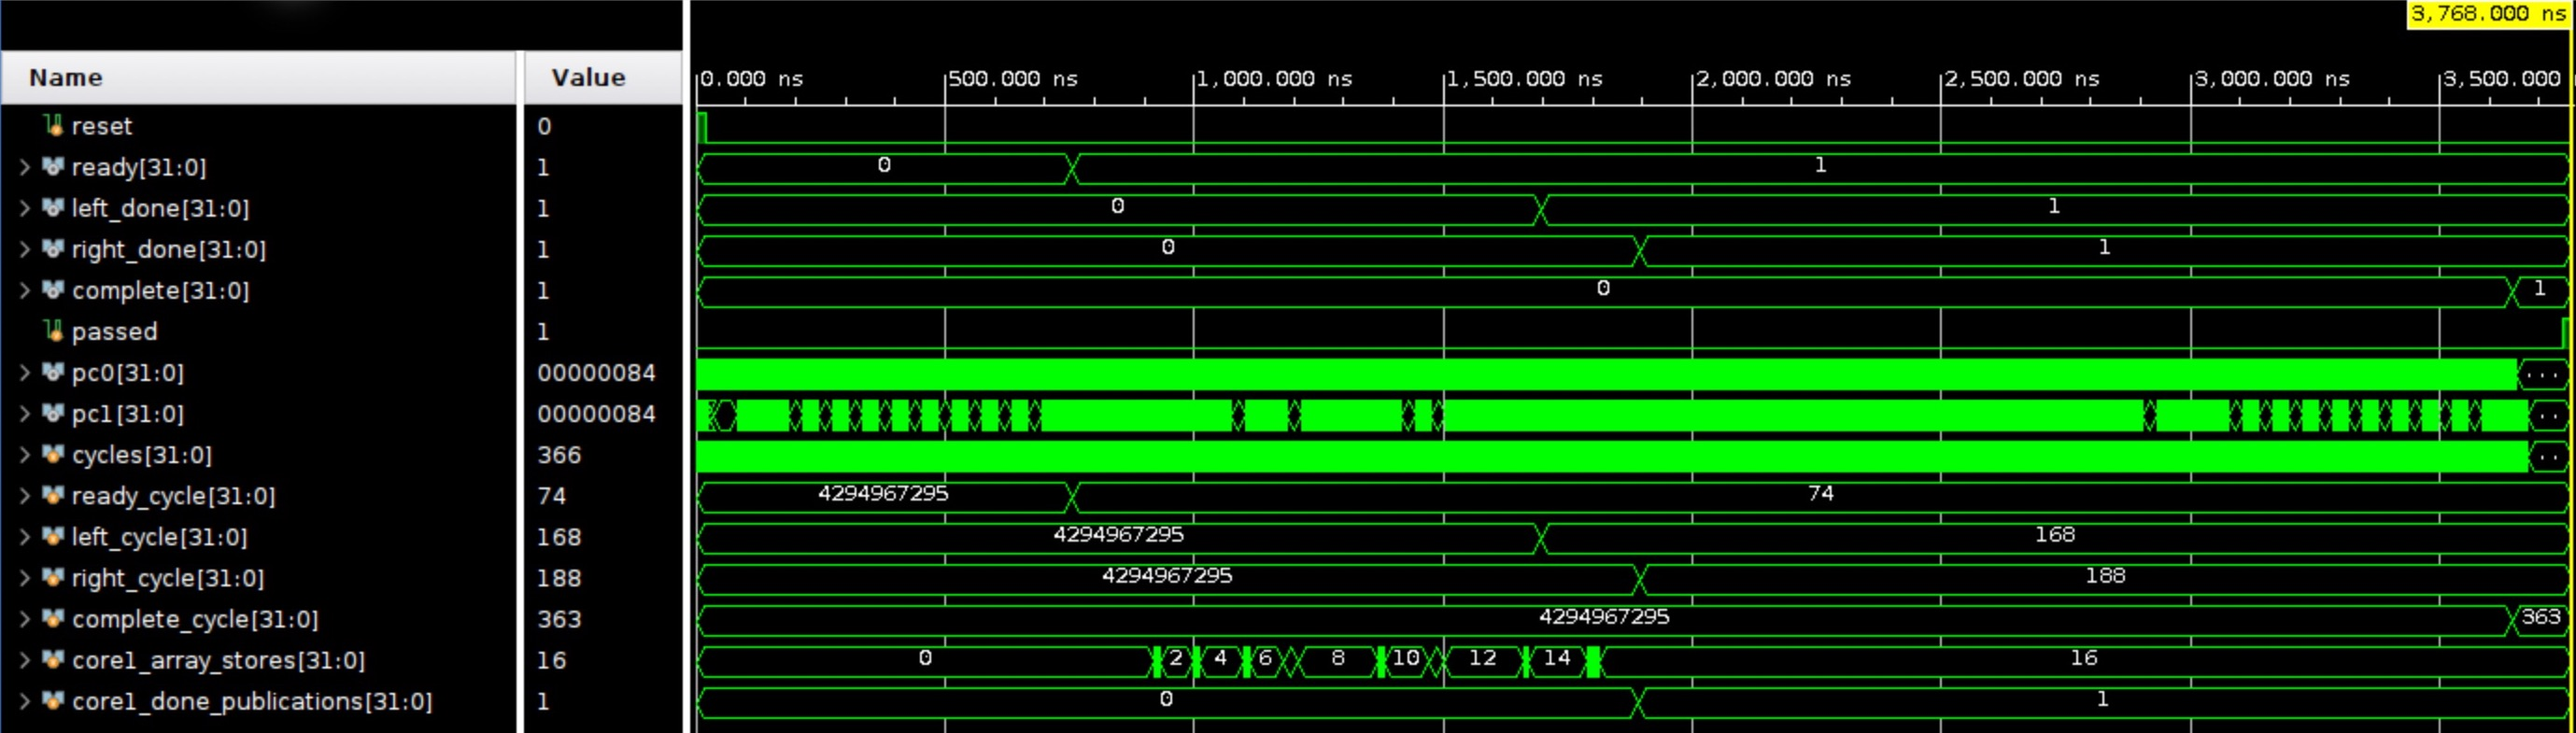
\includegraphics[bb=0 0 2758 785,viewport=0 403 410 785,clip,width=.261\linewidth]{figures/02-synchronization-wave.png}%
\hspace{.005\linewidth}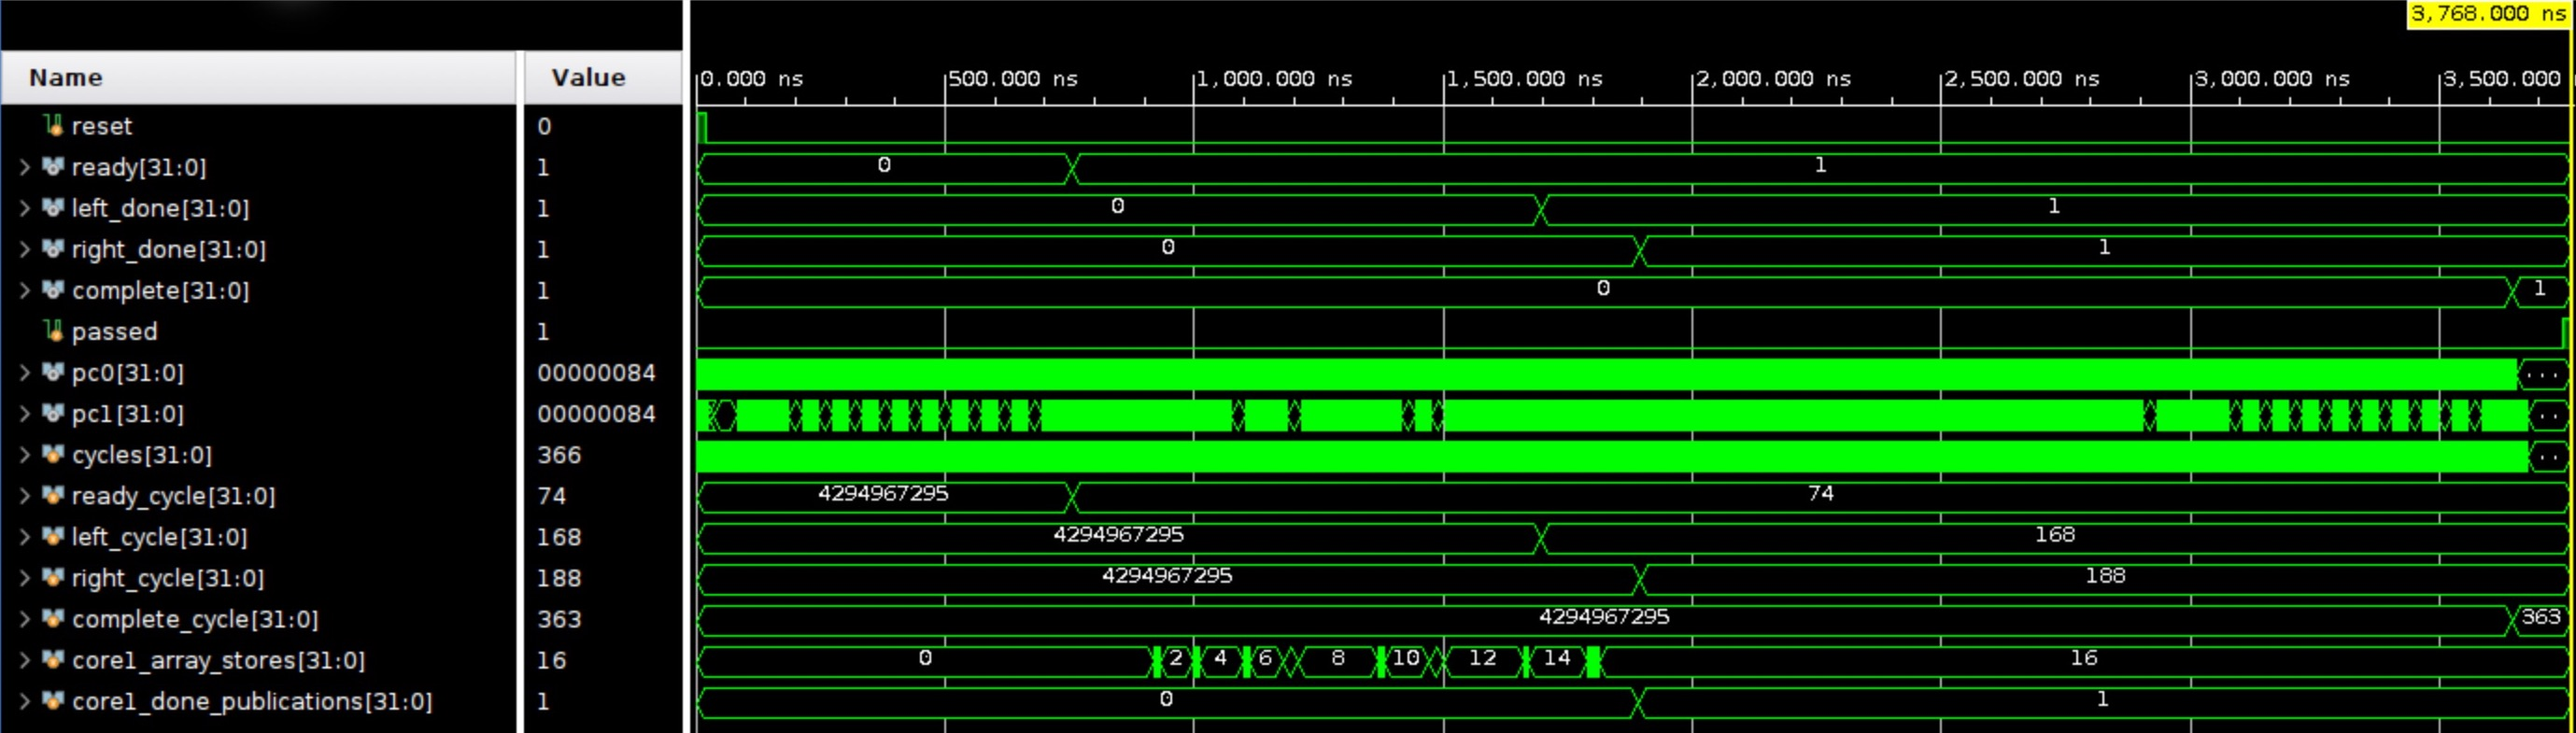
\includegraphics[bb=0 0 2758 785,viewport=555 403 675 785,clip,width=.076\linewidth]{figures/02-synchronization-wave.png}%
\hspace{.005\linewidth}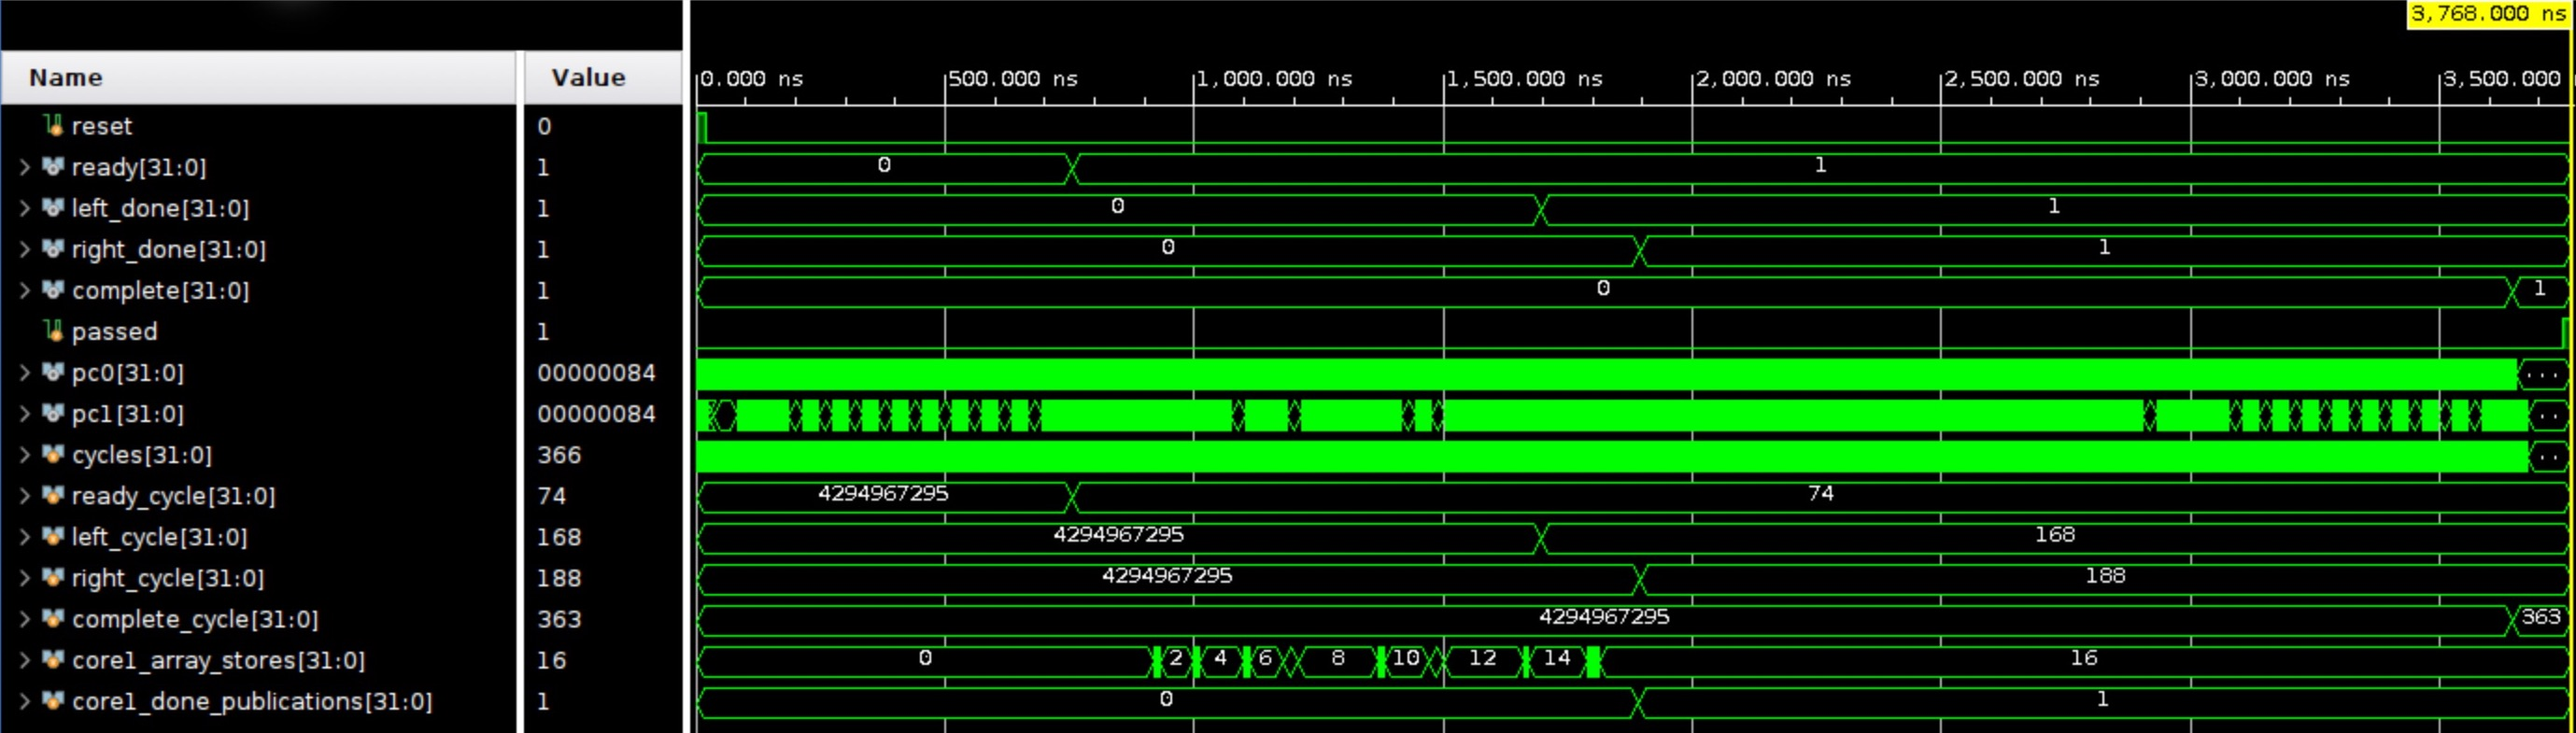
\includegraphics[bb=0 0 2758 785,viewport=742 403 1750 785,clip,width=.643\linewidth]{figures/02-synchronization-wave.png}\par\medskip

\noindent\makebox[\linewidth][l]{\small (b) 約1,900 ns〜終了}\par\smallskip

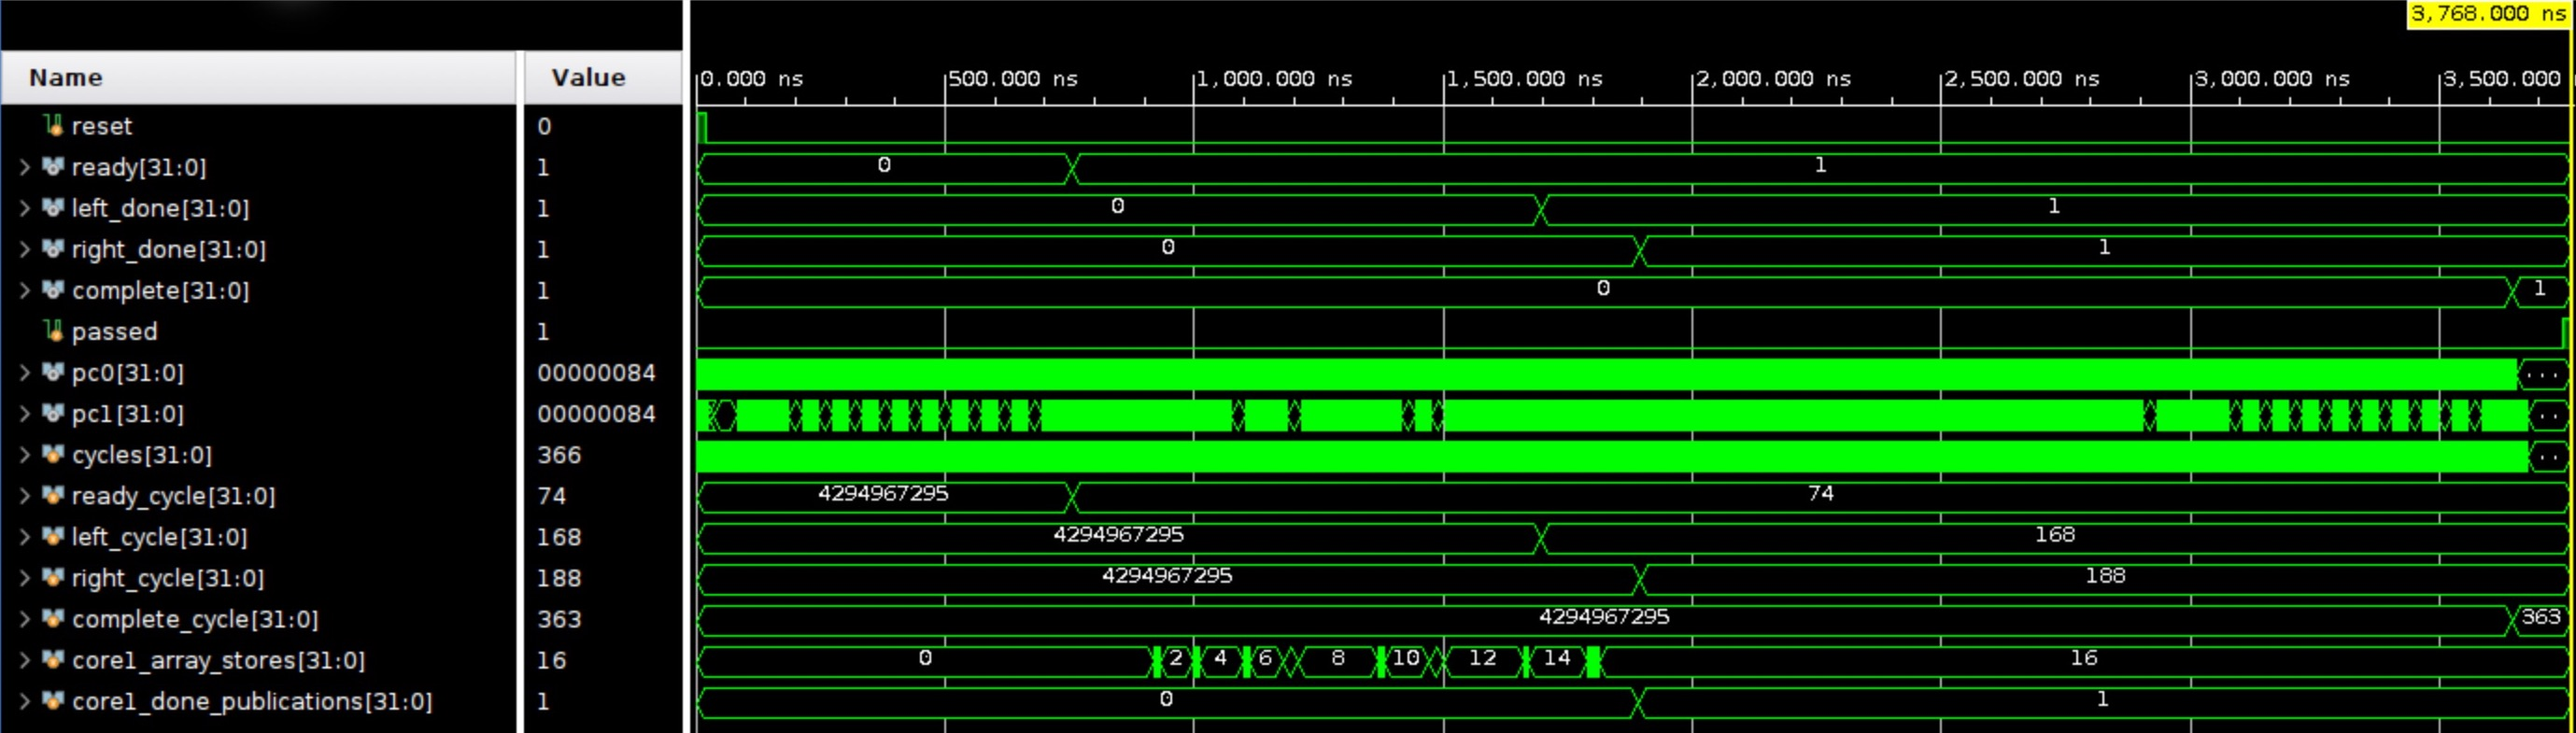
\includegraphics[bb=0 0 2758 785,viewport=0 403 410 785,clip,width=.261\linewidth]{figures/02-synchronization-wave.png}%
\hspace{.005\linewidth}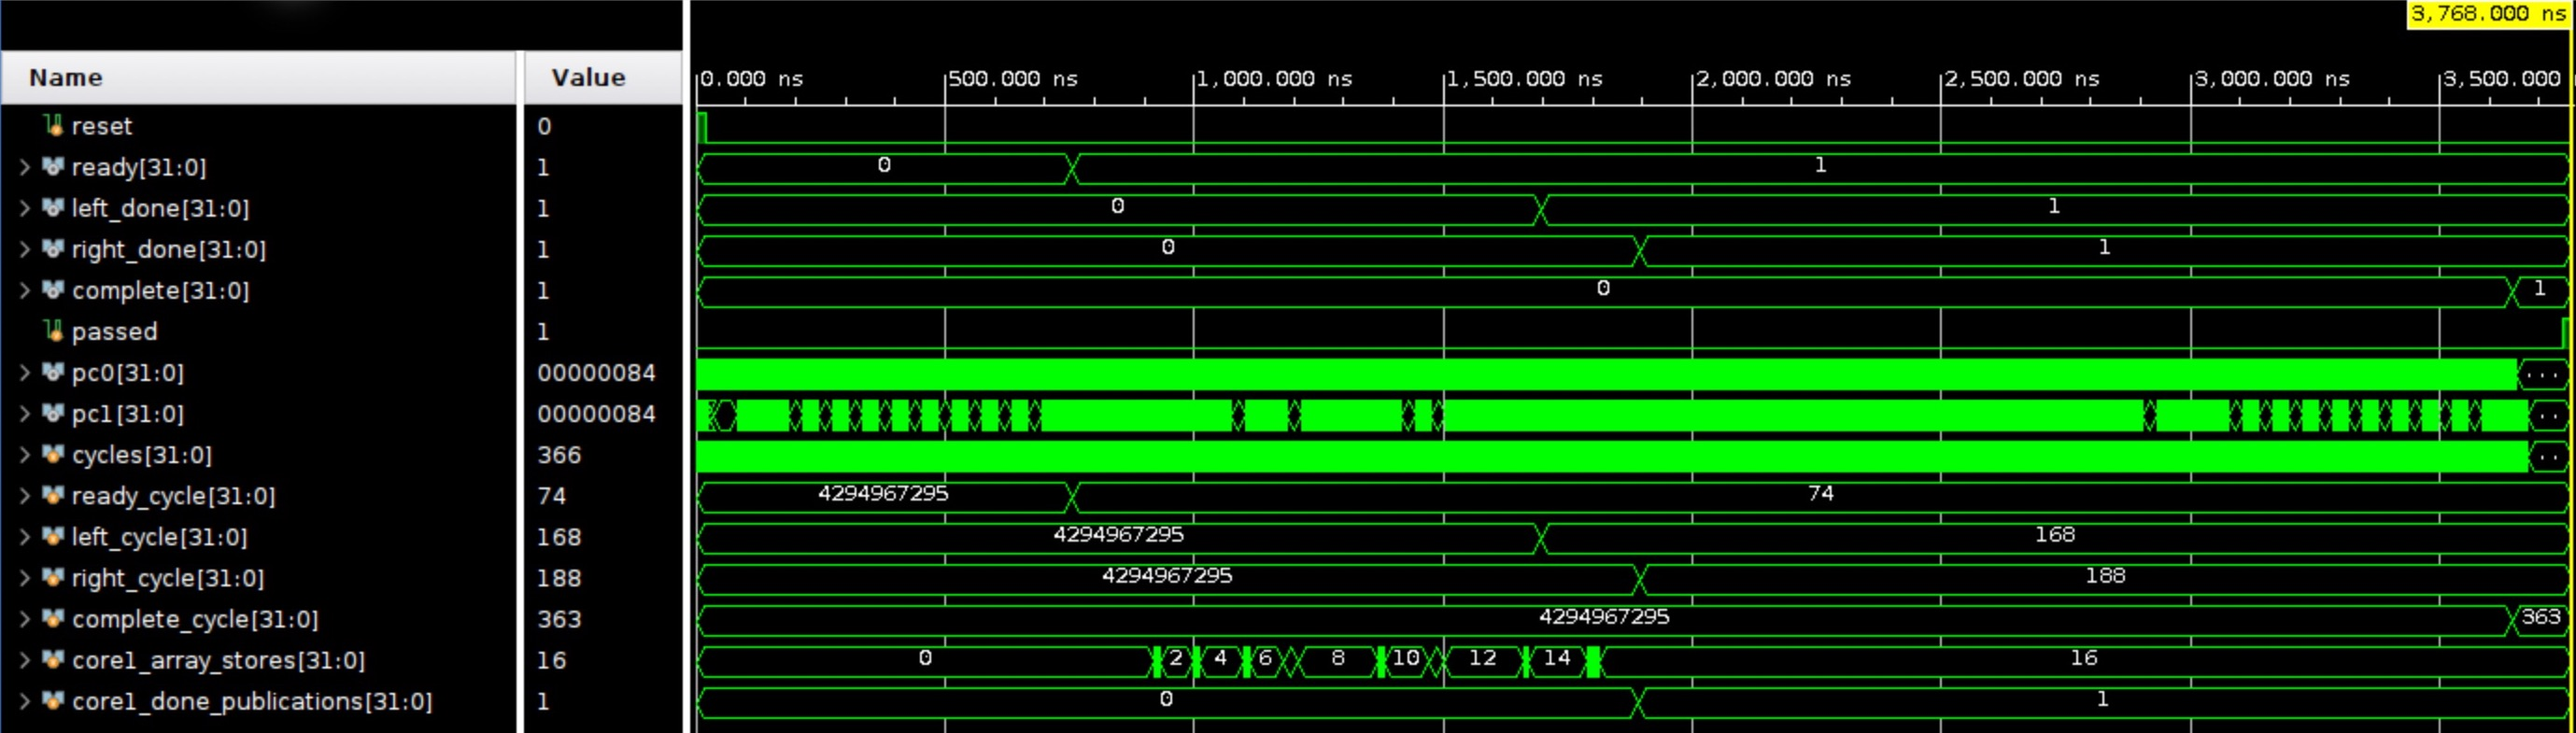
\includegraphics[bb=0 0 2758 785,viewport=555 403 675 785,clip,width=.076\linewidth]{figures/02-synchronization-wave.png}%
\hspace{.005\linewidth}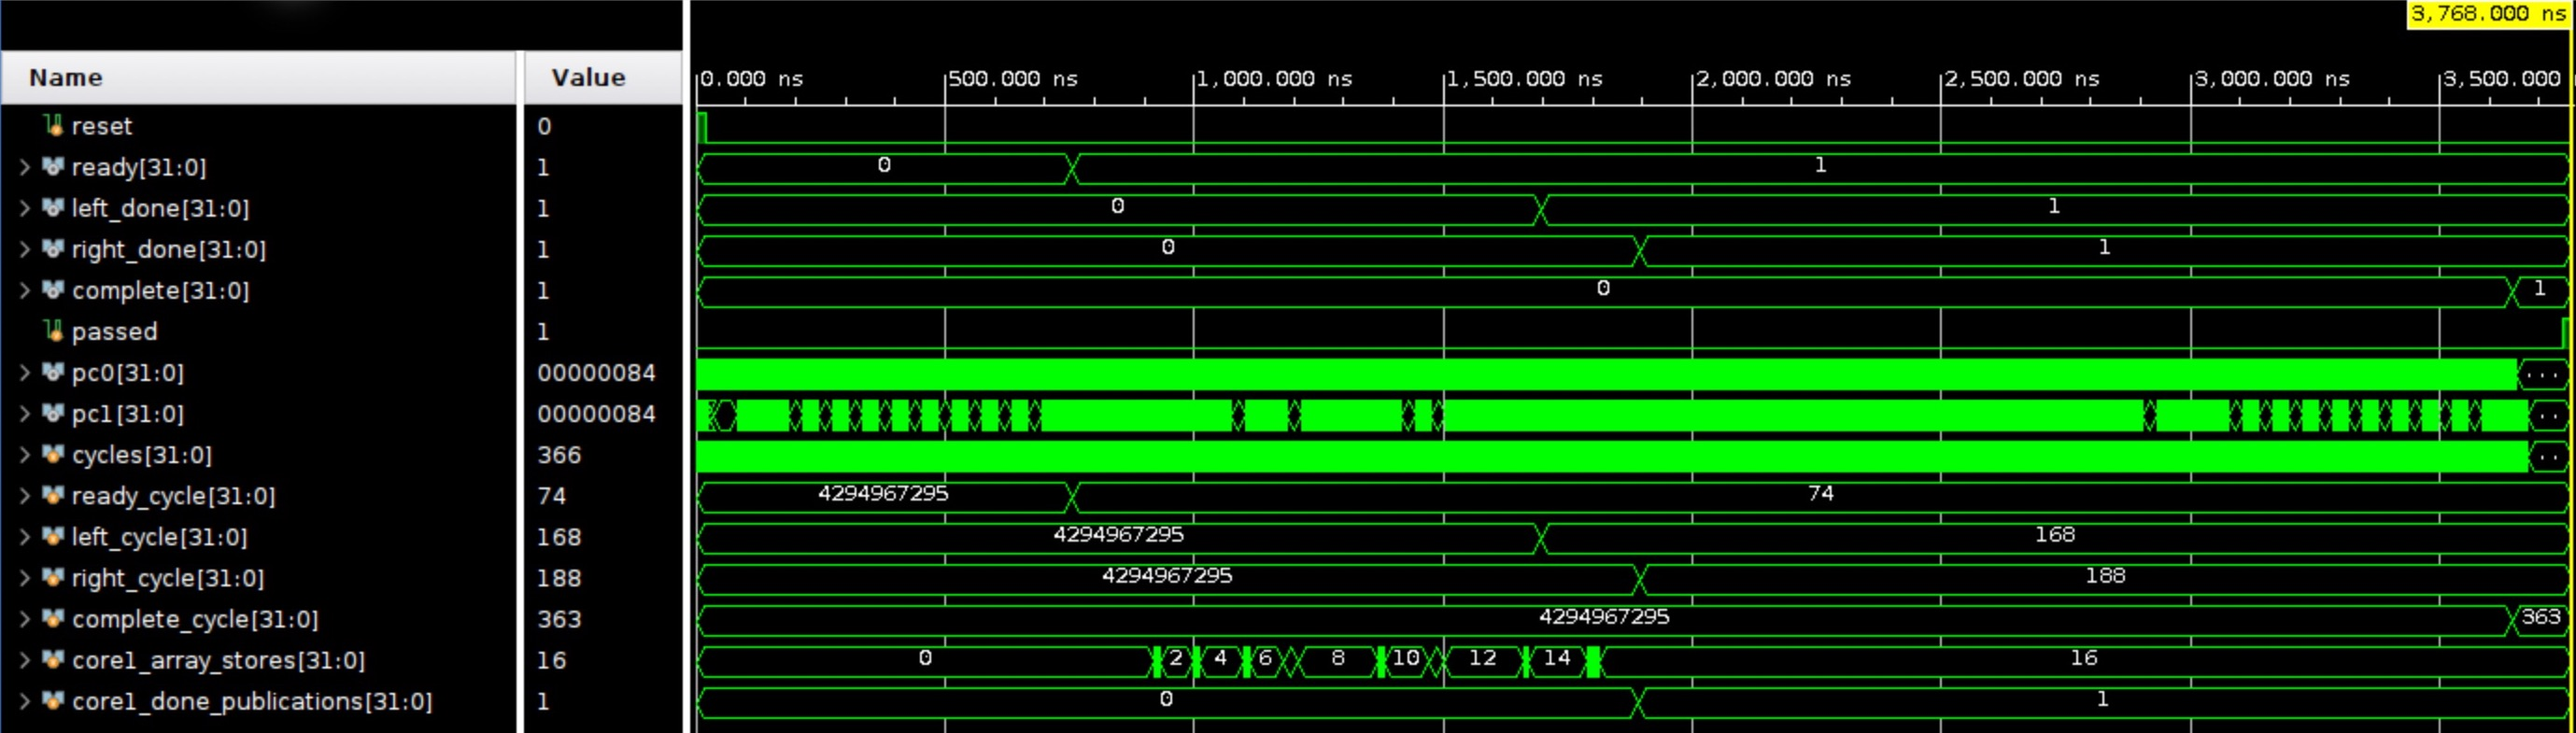
\includegraphics[bb=0 0 2758 785,viewport=1750 403 2758 785,clip,width=.643\linewidth]{figures/02-synchronization-wave.png}\par\medskip

\caption{10要素dual実行の完了フラグ。上下は同じ実行の前半と後半で、信号名を繰り返した。Value列は最終カーソル時点の値。横軸nsとリセット解除基準のcyclesは原点が異なる。}\label{fig:3}

\end{figure}

\begin{table}[H]

\centering

\caption{図3に対応する初回観測サイクル}

\label{tab:4}

\footnotesize

\setlength{\tabcolsep}{3pt}

\renewcommand{\arraystretch}{1.25}

\begin{tabular}{>{\raggedright\arraybackslash}p{\dimexpr0.180261\linewidth-2\tabcolsep\relax}>{\raggedright\arraybackslash}p{\dimexpr0.208302\linewidth-2\tabcolsep\relax}>{\raggedright\arraybackslash}p{\dimexpr0.208302\linewidth-2\tabcolsep\relax}>{\raggedright\arraybackslash}p{\dimexpr0.202293\linewidth-2\tabcolsep\relax}>{\raggedright\arraybackslash}p{\dimexpr0.200842\linewidth-2\tabcolsep\relax}}\toprule

\textbf{READY} & \textbf{LEFT\_DONE} & \textbf{RIGHT\_DONE} & \textbf{COMPLETE} & \textbf{参加コア終端}\\\midrule

74 & 168 & 188 & 363 & 366\\

\bottomrule\end{tabular}

\end{table}

波形では、左側の完了が168サイクル目、右側の完了が188サイクル目に観測された（図\ref{fig:3}、表\ref{tab:4}）。
Core0は右側の完了を確認してからマージと書き戻しを行い、363サイクル目にCOMPLETEを立てた。Core1がこれを確認し、参加コアが終端に達するまでを数えると366サイクルだった。



Core1による配列への書込みは16回受理され、右側の完了通知もCore1が1回書き込んだ。書込み先が担当区間内であることと、通知元がCore1であることはテストベンチで照合した（付録C）。



\section{競合時の状態保持と実行再開}\label{sec:4-3}

\par\medskip\noindent\begin{minipage}{\linewidth}
\par\medskip\noindent{\small\bfseries コード5a　Core0優先の調停とストール　simple\_memory\_arbiter.v}\par\nopagebreak

\lstinputlisting{code/code-05.txt}
\end{minipage}\par\medskip

req0とreq1が同時に1になると、Core0が許可され、Core1のstall1が1になる。
CPU側ではRegWriteを!stallで抑止し、PCも!stallのときだけ更新する。
この機構は既存のCPUから引き継いだ。



\par\medskip\noindent\begin{minipage}{\linewidth}
\par\medskip\noindent{\small\bfseries コード5b　レジスタ書込みとPC更新の抑止　simple\_cpu\_with\_mem\_interface.v}\par\nopagebreak

\lstinputlisting{code/code-06.txt}
\end{minipage}\par\medskip

\par\medskip\noindent\begin{minipage}{\linewidth}
\par\medskip\noindent{\small\bfseries コード6　隣接要素の比較と交換　listing.s}\par\nopagebreak

\lstinputlisting{code/code-07.txt}
\end{minipage}\par\medskip

このCPUのsltは符号なし比較である。
後ろの要素の値が小さければ、74〜75行で二つの要素を交換する。



\begin{figure}[H]

\centering

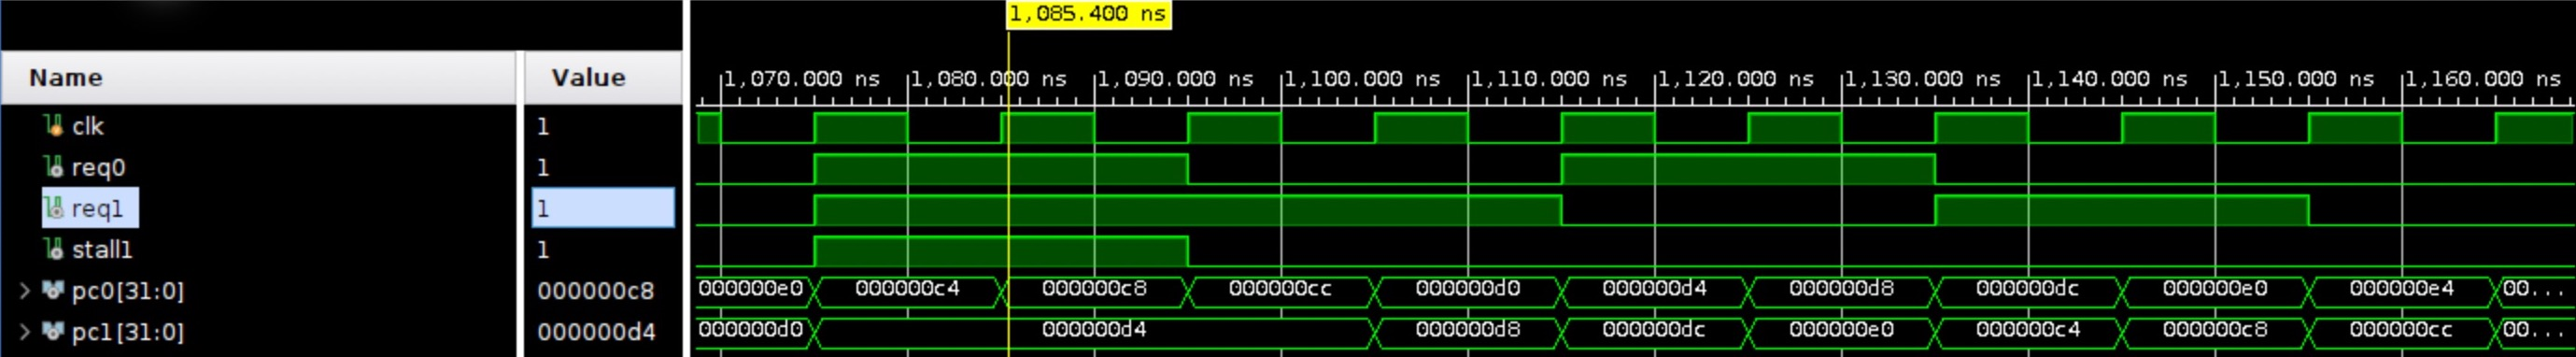
\includegraphics[bb=0 0 2758 382,viewport=0 0 1950 382,clip,width=\linewidth]{figures/03-contention-wave.png}

\caption{1085.4 ns付近の同時要求。req0、req1、stall1が1で、PC0は0xC8、PC1は0xD4を示す。Core1のPCは競合区間をまたいで保持され、待機解除後に0xD8へ進む。}\label{fig:4}

\end{figure}

付録AのPC注記と照合すると、0xC8はコード6の71行目のload、0xD4は74行目の最初のstoreである。
図\ref{fig:4}ではCore1のPCが1075〜1095 nsの競合区間をまたいで0xD4に留まる。
再開後の0xD8は75行目の次のstoreに対応する。



この実行でCore1がストールしたのは計77サイクルだった。図\ref{fig:4}ではその一例としてPCの保持と再開を示す。
テストベンチでは、ストールしたクロック端の前後でPCと全32レジスタを照合した（付録C.2）。



\section{マージ処理と最終配列の確認}\label{sec:4-4}

両側の完了後、Core0は整列済み区間の先頭を比較し、小さい値を0x1300からの作業領域へ書く。
同値では左側を選ぶ。
一方の区間を使い切ったら残りを転送し、作業領域の10要素を0x1100へ書き戻す。
付録Aに分岐と残り要素の処理を含む一覧を示す。



\par\medskip\noindent\begin{minipage}{\linewidth}
\par\medskip\noindent{\small\bfseries コード7　マージの比較と最後の書き戻し　listing.s}\par\nopagebreak

\lstinputlisting{code/code-08.txt}
\end{minipage}\par\medskip

\begin{figure}[H]

\centering

\begin{minipage}{.43\linewidth}

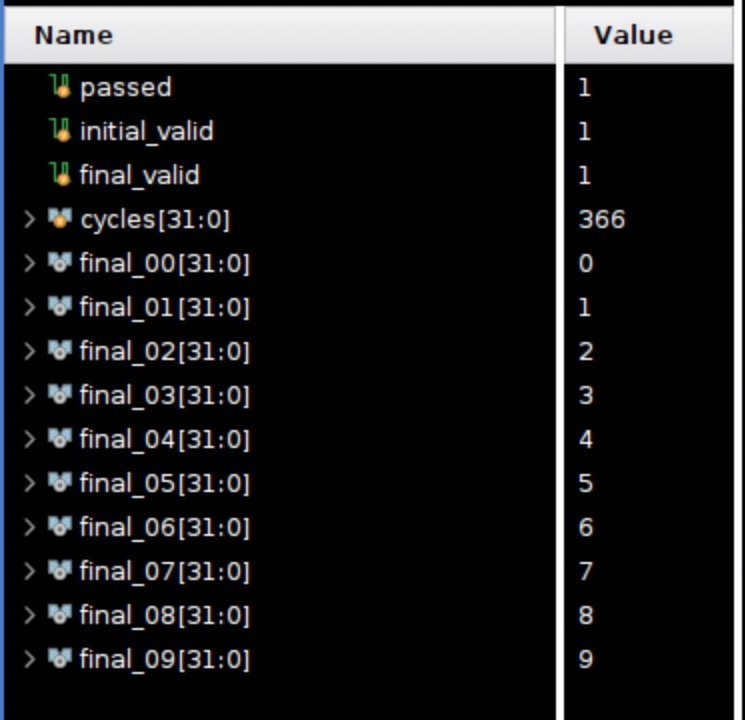
\includegraphics[width=\linewidth]{figures/01a-correctness-values.png}

\end{minipage}\hfill\begin{minipage}{.51\linewidth}

\small 入力\par 7,1,4,9,3,8,2,6,5,0\par \par 出力\par 0,1,2,3,4,5,6,7,8,9\par \par Core1の受理された配列storeは16回。自分の完了通知は1回だった。

\end{minipage}

\caption{最終スナップショット。final\_00〜final\_09は0〜9、cyclesは366。initial\_validは入力コピーの照合、final\_validは最終値の取得、passedは検査通過を示す。}\label{fig:5}

\end{figure}

\par\medskip\noindent\begin{minipage}{\linewidth}
\par\medskip\noindent{\small\bfseries コード8　保存した最終値と検査通過の公開　tb\_vivado\_sort.v}\par\nopagebreak

\lstinputlisting{code/code-09.txt}
\end{minipage}\par\medskip

図\ref{fig:5}は同じten-dual-v2実行の波形で、マージ後の配列が0から9まで昇順に並んでいる。
final\_validは最終値を取り込んだこと、passedは期待値との照合を含む検査を通過したことを示す。
この波形に表示したのはマージ後の配列で、左右それぞれのソート直後の配列ではない。



\chapter{検証結果}\label{chap:5}

本章では、全54条件を対象とした機能検証の結果、および追加検証・異常系テストの結果を報告する。
続いて、代表入力に対する1コア実行と2コア実行の総サイクル数を比較し、要素数や方式による傾向を示す。

\section{出力と途中状態の検査結果}\label{sec:5-1}

18種類の入力ケースに対して3つの実行方式を適用した計54条件についてシミュレーションを実施した結果、すべての条件で最終配列が期待値と完全に一致し、\ref{sec:3-3}節で述べた実行途中の各種検査を通過した。
各条件の実行ログにおけるPASS出力および終了コード0の確認結果は、総サイクル数とあわせて付録\ref{chap:B}にまとめる。
また、指定10要素をdual方式で実行した際の詳細な波形は、前章の図\ref{fig:3}〜\ref{fig:5}に示したとおりである。

主検証の54条件に加えて、補助的な動作確認も実施した。
具体的には、指定10要素および乱数64要素を各3方式で実行した計6件の波形デモと、コアID読み出し、既存のマルチコア基本動作、ROM読み出し時の競合、およびメモリ配置を対象とした計4件の単体検証を実施し、いずれも正常に通過することを確認した。
これらは主検証の54条件とは独立した実行記録であり、波形デモの入力ケースは主検証と共通である。

さらに、テストベンチの期待値照合が異常を確実に検出できることを確認するため、意図的に誤った期待値を与えた異常系テストを実行した。
このテストでは、array[0]の期待値0xFFFFFFFFに対して実際の出力値が0x00000000である不一致を検出し、終了コード1で実行を停止した。
単一の異常系テストのみで検査器の全エラー経路を網羅できるわけではないが、最終配列の不一致検出機能が意図どおりに働くことを確認できた。

\section{1コア・2コア実行の総サイクル数比較}\label{sec:5-2}

表\ref{tab:5}に、代表入力における各方式の総サイクル数およびserial\_splitとdualのサイクル比を示す。
主比較である1コア逐次分割方式（serial\_split）と2コア並列方式（dual）を比べると、指定10要素では442サイクルから366サイクルへ短縮された（比1.21）。
固定乱数の4ケースでは、サイクル比が7要素の1.08から64要素の1.56へと拡大しており、要素数が増えるにつれて並列実行の短縮効果が顕著になる傾向が確認された。
ただし、各要素数につき1種類の固定配列のみを評価しているため、入力の並び順による変動と要素数による効果は厳密には分離されていない。

\begin{table}[H]
\centering
\caption{代表入力における各方式の総サイクル数}
\label{tab:5}
\footnotesize
\setlength{\tabcolsep}{3pt}
\renewcommand{\arraystretch}{1.25}
\begin{tabular}{>{\raggedright\arraybackslash}p{\dimexpr0.150218\linewidth-2\tabcolsep\relax}>{\raggedright\arraybackslash}p{\dimexpr0.216313\linewidth-2\tabcolsep\relax}>{\raggedright\arraybackslash}p{\dimexpr0.170247\linewidth-2\tabcolsep\relax}>{\raggedright\arraybackslash}p{\dimexpr0.190276\linewidth-2\tabcolsep\relax}>{\raggedright\arraybackslash}p{\dimexpr0.272947\linewidth-2\tabcolsep\relax}}\toprule
\textbf{入力} & \textbf{serial\_split} & \textbf{dual} & \textbf{split/dual} & \textbf{参考 serial\_full}\\\midrule
指定10 & 442 & 366 & 1.21 & 441\\
乱数7 & 281 & 260 & 1.08 & 230\\
乱数17 & 923 & 733 & 1.26 & 1,164\\
乱数32 & 2,513 & 1,772 & 1.42 & 3,763\\
乱数64 & 8,614 & 5,527 & 1.56 & 14,803\\
\bottomrule\end{tabular}
\end{table}

一方、参考条件であるserial\_fullとの比較では、要素数が小さい乱数7においてserial\_fullの230サイクルに対しdualが260サイクルと30サイクル上回った。
これは、要素数が少ない領域では分割とマージおよび同期の固定的なオーバーヘッドがバブルソート自体の処理量に対して大きく影響するためである。
逆に17要素以上では配列分割による比較回数の削減効果が上回り、dualとserial\_splitのいずれもserial\_fullより少ないサイクル数となった。
もっとも、serial\_fullはマージを伴わない点でアルゴリズム構成が異なるため、この差を単純にコア数のみの効果として解釈すべきではない。

\chapter{サイクル数に関する考察}\label{chap:6}

\section{処理区間別のサイクル数}\label{sec:6-1}

固定乱数64要素では、8,614から5,527サイクルに減った（35.8\%減）。
READYまでの398サイクルは両方式で同じだった。差がついたのは主にREADYから両側のソートが終わるまでで、この区間は7,178から4,087サイクルになった（表\ref{tab:6}）。



\begin{table}[H]

\centering

\caption{乱数64要素のイベント間サイクル数}

\label{tab:6}

\footnotesize

\setlength{\tabcolsep}{3pt}

\renewcommand{\arraystretch}{1.25}

\begin{tabular}{>{\raggedright\arraybackslash}p{\dimexpr0.566821\linewidth-2\tabcolsep\relax}>{\raggedright\arraybackslash}p{\dimexpr0.216313\linewidth-2\tabcolsep\relax}>{\raggedright\arraybackslash}p{\dimexpr0.216865\linewidth-2\tabcolsep\relax}}\toprule

\textbf{観測区間} & \textbf{serial\_split} & \textbf{dual}\\\midrule

開始からREADY & 398 & 398\\

READYから両側ソート完了 & 7,178 & 4,087\\

両側完了からCOMPLETE & 1,037 & 1,039\\

COMPLETEから参加コア終端 & 1 & 3\\

総サイクル数 & 8,614 & 5,527\\

\bottomrule\end{tabular}

\end{table}

両側のソート完了からCOMPLETEまでは、1コアで1,037、2コアで1,039サイクルとほぼ同じだった。この区間にはマージと書き戻しに加え、フラグの確認と通知も含まれる。
初期コピーやマージはCore0が担当し、並行ソート中にも共有ポートの待ちがあるため、2コアでも総サイクル数は1コアの半分にはならない。



\section{入力配列・交換回数と総サイクル数}\label{sec:6-2}

\begin{table}[H]

\centering

\caption{64要素の2コア実行を入力別に比較}

\label{tab:7}

\footnotesize

\setlength{\tabcolsep}{3pt}

\renewcommand{\arraystretch}{1.25}

\begin{tabular}{>{\raggedright\arraybackslash}p{\dimexpr0.158229\linewidth-2\tabcolsep\relax}>{\raggedright\arraybackslash}p{\dimexpr0.160232\linewidth-2\tabcolsep\relax}>{\raggedright\arraybackslash}p{\dimexpr0.218316\linewidth-2\tabcolsep\relax}>{\raggedright\arraybackslash}p{\dimexpr0.266386\linewidth-2\tabcolsep\relax}>{\raggedright\arraybackslash}p{\dimexpr0.196836\linewidth-2\tabcolsep\relax}}\toprule

\textbf{入力} & \textbf{総数} & \textbf{両側完了\newline の時点} & \textbf{両側完了から\newline COMPLETE} & \textbf{Core1\newline ストール}\\\midrule

整列 & 4,398 & 3,481 & 914 & 388\\

逆順 & 5,391 & 4,473 & 915 & 389\\

乱数 & 5,527 & 4,485 & 1,039 & 925\\

\bottomrule\end{tabular}

\end{table}

乱数64要素は逆順64要素より136サイクル長い。
左右のソートが終わったのは、乱数入力で4,485サイクル目、逆順入力で4,473サイクル目で、差は12サイクルだった。そこからCOMPLETEまでにそれぞれ1,039サイクルと915サイクルを要し、この区間だけで124サイクルの差がついた。
差の大半は後段に現れており、ストール数だけでは総数を説明できない。



マージでは、左右の値の並びで比較回数や残り要素の転送が変わる。ただし後段にはフラグの確認と通知も含まれるため、124サイクルすべてがマージによる差とは言えない。
Core1のストール中にもCore0は動けるので、ストール回数をそのまま総サイクル数の増分として扱わない。



整列済み入力でも比較走査を続ける実装のため、4,398サイクルを要した。
Core1による配列へのstoreは、整列済み入力で0回、逆順入力で992回、乱数入力で468回だった。storeが最も多かったのは逆順入力だが、総サイクル数が最も多かったのは乱数入力だった。
ソート中の交換回数に加え、待機と後段処理を含む総数を見る必要がある。



\chapter{結論と限界}\label{chap:7}

本章では、本報告における設計統合と検証から得られた知見を総括し、現在の検証範囲および未検証事項を整理する。
最後に、再現性を確保するための検証対象バージョンと根拠資料の対応を示す。

\section{検証で得られた知見}\label{sec:7-1}

本報告では、既存の2コアCPUに入力ROMのデータ読み出し経路とコアIDの互換アドレスを統合し、共有メモリ上での分割バブルソートの動作とサイクル数をXSim 2023.1で検証した。
選定した18種類の入力ケース（計54条件）すべてにおいて、共有データポートを調停しながらCore0・Core1が各担当区間を並行してソートし、両側の完了同期を経てCore0が正しくマージを完了することを確認した。
さらに、10要素の代表入力に関する波形解析により、競合発生時のCore1のストールとPC保持、待機解除後の実行再開、完了フラグの推移、および最終配列出力に至る一連の挙動を実コードと対応付けて実証した。

サイクル数の比較分析では、同一アルゴリズムを1コアで逐次実行する場合（serial\_split）に比べ、2コア実行（dual）は指定10要素で442から366サイクルへ、固定乱数64要素で8,614から5,527サイクル（35.8\%減）へと短縮された。
処理区間ごとの内訳から、短縮効果の大半はREADYから両側ソート完了までの並行区間に集中している一方、初期コピーおよびマージ・書き戻しを含む逐次区間はほぼ変わらず、共有ポート競合とあわせて2倍速に達しない主要因となっていることが明らかになった。

\section{検証範囲と未検証事項}\label{sec:7-2}

本検証にはいくつかの前提と限界がある。
機能検証の対象は、リセットおよびメモリ初期化後の状態から起動し、選定した最大64要素の符号なし32ビット入力を処理する条件に限られる。
したがって、前回実行のフラグが残存した状態からの再起動、64要素を超える大規模入力、Core0固定優先調停のもとでCore1が長時間待たされる状況、複数の乱数シードによるサイクル数のばらつき、ならびに検査コードのカバレッジ評価は今後の検証課題として残されている。

また、本報告の性能評価はすべてRTLビヘイビアシミュレーション上のサイクル数に基づくものであり、論理合成、配置配線、およびFPGA実機での動作測定は行っていない。
実機における処理時間の短縮率はサイクル数の比だけでなく最大動作周波数にも依存するため、非同期読み出しメモリのFPGA資源への実装方法、回路規模、およびタイミング制約を含めた実機評価が別途必要である。

\section{検証対象の版と根拠資料}\label{sec:7-3}

本報告の検証対象は、原本リポジトリtakehaya/antikytheraの未コミット変更を含む作業状態（HEAD:\ \allowbreak 8b61da20522f5bfcb01908f2342abfea7676bb25）を出発点とし、第\ref{chap:2}章の統合変更を加えた版である。
そのため、HEADコミット単体からは同一の検証環境を再現できない。
参照した全19ファイルの一覧とSHA-256ハッシュ値はsource-manifest.jsonに記録しており、ファイル集合識別子の先頭16桁は62eb51779b0c0173である。

表\ref{tab:8}に本文の記述と保存資料の対応をまとめる。
原本リポジトリは文献\cite{antikythera}に、Vivadoシミュレーションおよび波形操作の参照資料は文献\cite{ug900,ug835}に示す。
なお、参照した公式マニュアルは2020.2版であり、本報告の実測に用いた実行環境（XSim 2023.1）とは版が異なる。

\begin{table}[H]
\centering
\caption{本文の根拠と保存資料の対応}
\label{tab:8}
\footnotesize
\setlength{\tabcolsep}{3pt}
\renewcommand{\arraystretch}{1.25}
\begin{tabular}{>{\raggedright\arraybackslash}p{\dimexpr0.340493\linewidth-2\tabcolsep\relax}>{\raggedright\arraybackslash}p{\dimexpr0.659507\linewidth-2\tabcolsep\relax}}\toprule
\textbf{根拠項目} & \textbf{保存資料}\\\midrule
実装と命令一覧 & work/内のRTL、tests/sort/build\_programs.py、research/cases/original\_ten/dual/listing.s\\
54条件の数値・判定 & report/xsim-results.csv、runs/matrix-*/simulate.logおよび終了記録\\
図\ref{fig:3}〜\ref{fig:5}の波形画面 & runs/ten-dual-v2/evidence.wdb、report/gui-captures-20261011/内の原本と切出し記録\\
途中状態の検査コード & tests/sort/tb\_sort.v、research/sim/tb\_vivado\_sort.v\\
\bottomrule\end{tabular}
\end{table}

\renewcommand{\bibname}{参考文献}
\renewcommand{\em}{\it}
\bibliographystyle{jplain}
\bibliography{reference}
\appendix

\chapter{10要素の2コア実行プログラム}\label{chap:A}

research/cases/original\_ten/dual/listing.sの実ファイルを行番号付きで掲載する。
右側の注記は命令のPCと機械語である。
この一覧を使うと、図\ref{fig:4}のPCがどの命令を指すか分かる。
長いコメントは紙面内で折り返す。



\par\medskip\noindent{\small\bfseries コードA1　起動、分担、完了待機（1〜45行）}\par\nopagebreak

\lstinputlisting{code/code-10.txt}

\section*{コピー処理とバブルソート}

\par\medskip\noindent{\small\bfseries コードA2　コピー、比較交換、マージの入口（46〜89行）}\par\nopagebreak

\lstinputlisting{code/code-11.txt}

70〜75行の比較交換は両コアで共通である。
走査範囲を1要素ずつ縮める固定パスを使い、交換がなかったことによる早期終了は行わない。



\clearpage
\section*{マージ処理と入力データ}

\par\medskip\noindent{\small\bfseries コードA3　マージ、書き戻し、入力ROM（90行〜末尾）}\par\nopagebreak

\lstinputlisting{code/code-12.txt}

\setcounter{table}{0}\renewcommand{\thetable}{B\arabic{table}}

\chapter{全54条件の検証結果}\label{chap:B}

表の各行に、一つの入力群を3方式で実行したときの総サイクル数を示す。
18行×3方式の54条件について、既存simulate.logのPASS行と終了コード0を確認した。
入力の名前は保存済みケース名と一致させた。



\begin{table}[H]

\centering

\caption{18入力群、3方式の全結果}

\label{tab:B1}

\footnotesize

\setlength{\tabcolsep}{3pt}

\renewcommand{\arraystretch}{1.25}

\begin{tabular}{>{\raggedright\arraybackslash}p{\dimexpr0.340493\linewidth-2\tabcolsep\relax}>{\raggedright\arraybackslash}p{\dimexpr0.056081\linewidth-2\tabcolsep\relax}>{\raggedright\arraybackslash}p{\dimexpr0.156226\linewidth-2\tabcolsep\relax}>{\raggedright\arraybackslash}p{\dimexpr0.124180\linewidth-2\tabcolsep\relax}>{\raggedright\arraybackslash}p{\dimexpr0.154223\linewidth-2\tabcolsep\relax}>{\raggedright\arraybackslash}p{\dimexpr0.168796\linewidth-2\tabcolsep\relax}}\toprule

\textbf{ケース名} & \textbf{N} & \textbf{serial\_split} & \textbf{dual} & \textbf{serial\_full} & \textbf{判定}\\\midrule

empty & 0 & 49 & 46 & 27 & 全3方式PASS\\

singleton\_zero & 1 & 67 & 64 & 33 & 全3方式PASS\\

singleton\_max & 1 & 67 & 64 & 33 & 全3方式PASS\\

sorted\_two & 2 & 89 & 86 & 51 & 全3方式PASS\\

reverse\_two & 2 & 90 & 87 & 53 & 全3方式PASS\\

duplicate\_three & 3 & 123 & 122 & 74 & 全3方式PASS\\

original\_ten & 10 & 442 & 366 & 441 & 全3方式PASS\\

sorted\_ten & 10 & 399 & 321 & 387 & 全3方式PASS\\

reverse\_ten & 10 & 440 & 342 & 477 & 全3方式PASS\\

duplicate\_ten & 10 & 443 & 367 & 437 & 全3方式PASS\\

equal\_sixteen & 16 & 753 & 558 & 891 & 全3方式PASS\\

uint32\_nine & 9 & 388 & 344 & 364 & 全3方式PASS\\

random\_seven & 7 & 281 & 260 & 230 & 全3方式PASS\\

random\_seventeen & 17 & 923 & 733 & 1,164 & 全3方式PASS\\

random\_thirtytwo & 32 & 2,513 & 1,772 & 3,763 & 全3方式PASS\\

sorted\_sixtyfour & 64 & 7,473 & 4,398 & 12,699 & 全3方式PASS\\

reverse\_sixtyfour & 64 & 9,458 & 5,391 & 16,731 & 全3方式PASS\\

random\_sixtyfour & 64 & 8,614 & 5,527 & 14,803 & 全3方式PASS\\

\bottomrule\end{tabular}

\end{table}

出典はreport/xsim-results.csvと各実行ログである。
CSVにはサイクル数などの観測値が入り、PASS判定は実行ログと終了記録で確認する。
波形デモ6件と追加検証4件、期待値不一致の負例は、この54条件には加算していない。



\chapter{途中状態と終了時の検査コード}\label{chap:C}

本付録では、\ref{sec:3-3}節で述べた実行途中の動的検査および終了時の最終配列照合を実装したテストベンチ（tests/sort/tb\_sort.v）の主要部分を抜粋して示す。

\section{書き込み領域と完了通知の検査}\label{sec:C-1}

コードC1に示すとおり、テストベンチはストア命令が受理されるたびにcheck\_writeタスクを呼び出し、アドレスの正当性、担当区間外への書き込み、READY成立前の書き込み、および両側完了前のマージ開始を検査する。
あわせて、Core1による配列領域への受理書き込み回数およびRIGHT\_DONE通知回数を計数することで、最終配列の一致とは独立に並列分担の正当性を検証している。

\par\medskip\noindent{\small\bfseries コードC1　書き込み領域の検査とCore1受理書き込みの計数（tb\_sort.v）}\par\nopagebreak
\lstinputlisting{code/code-13.txt}

\clearpage
\section{ストール時のPC・レジスタ保持の検査}\label{sec:C-2}

共有ポート競合時の状態保持を確認するため、テストベンチはクロックエッジの直前に各コアのPC、全32レジスタを連結したall\_regs、およびストール信号を保存し、クロックエッジ後に再比較する（コードC2）。
これにより、図\ref{fig:4}の波形上で視認できるPCだけでなく、レジスタファイル全体の意図しない書き換えも漏れなく検出できる。

\par\medskip\noindent{\small\bfseries コードC2　ストール前後の状態保持検査（tb\_sort.v）}\par\nopagebreak
\lstinputlisting{code/code-14.txt}

\section{完了通知と最終配列の照合}\label{sec:C-3}

両コアが終端ループへ到達した後は、コードC3によってプロトコル上の全完了フラグが成立していること、各コアが自身の完了通知をちょうど1回ずつ行ったこと、および配列領域の64ワードが期待値と一致することを確認する。
加えて、188〜196行では配列領域の下端（0x10FC）および上端（0x1200）、作業領域の下端（0x12FC）、使用した作業領域直後の各ガードワードが0のままであることも検査している。
なお、入力コピー直後のスナップショット取得と図\ref{fig:5}の表示用フラグは、波形観測用のtb\_vivado\_sort.vにおいて追加実装したものである。

\par\medskip\noindent{\small\bfseries コードC3　終了条件の確認と最終配列64ワードの照合（tb\_sort.v）}\par\nopagebreak
\lstinputlisting{code/code-15.txt}

\end{document}
